%\documentclass{amsart}
%\usepackage[margin=0.75in]{geometry}
%\usepackage{microtype,hyperref,xcolor,graphicx,amssymb,ulem}
%\newcommand{\Z}{\mathbb{Z}}
%\newcommand{\R}{\mathbb{R}}
%\newcommand{\C}{\mathbb{C}}
%\renewcommand{\H}{\mathbb{H}}
%\renewcommand{\L}{\Lambda}
%\DeclareMathOperator{\zspan}{\ensuremath{\Z}-span}
%\def\vec{\mathbf}
%\def\mod{\bmod}
%\def\qedsymbol{\scriptsize\ensuremath\boxtimes}
%\DeclareMathOperator{\GL}{GL}
%\DeclareMathOperator{\vol}{vol}
%\newcommand{\pgram}{parallelogram}
%\newcommand{\ptope}{parallelotope}
%\newtheorem*{thm}{Theorem}
%\theoremstyle{definition}
%\newtheorem*{defn}{Definition}
%\newtheorem*{lem}{Lemma}
%\newtheorem*{claim}{Claim}
%\begin{document}
%\title{The Geometry of Numbers}
%\author{Dr. Brian Conrad\\July 11, 2012}
%\maketitle
\label{geoofnum}
The goal of this lecture is to illustrate the idea that geometric arguments in Euclidean space can be used to prove number-theoretic statements about integers. The phrase ``the geometry of numbers'' is originally due to Minkowski. In this lecture, a geometric argument will be used to prove the Lagrange Four-Square Theorem.

\begin{thm}[Lagrange Four-Square Theorem]
\label{foursquare}
Every natural number $n$ is of the form $n = x^2+y^2+z^2+w^2$, $x,y,z,w\in\Z$.
\end{thm}
Of course, some of these will have to be zero, as in $0 = 0^2+0^2+0^2+0^2$, $1 = 1^2 + 0^2+0^2+0^2$, and $2 = 1^2+1^2+0^2+0^2$. Additionally, four squares will be necessary, because any $n = 7\mod 8$ cannot be written as the sum of three squares (since the squares are $0,1,4\mod 8$).

The proof will be formulated geometrically in $\R^4$ and uses the rather unrelated fact that $\pi^2 > 8$. In this formulation, the theorem claims that every sphere $x^2+y^2+z^2+w^2 = n$ with $n$ a natural number intersects the lattice of integers $\Z^4 \subset\R^4$.

\begin{proof}
One can use Euler's identity, or
\[
\Bigg(\sum_{j=1}^4 x_j^2\Bigg)\left(\sum_{k=1}^4y_k^2\right) = \sum_{h=1}^4 B_n(\vec x,\vec y)^2
\]
where $B_n$ is some bilinear operation $B_n = \sum_{i,j=1}^4 \pm x_iy_i$, to show that a number is a sum of four squares if its prime factors are.

(This is motivated by the fact that the norm on $\C$ is commutative, so that for real $x,y,u,v$, \[(xu-yv)^2+(xv-yu)^2 = (x^2+y^2)(u^2+v^2).\] If this is generalized to the quarternions $\H$, then one obtains Euler's identity, which can be checked fairly straightforwardly by multiplying out. But it takes some insight to see beforehand --- and Euler himself had no conception of the quarternions.)

With $0,1,$ and $2$ shown above, then the only numbers for which the four-squares theorem needs to be checked are the odd primes. This doesn't seem particularly helpful, but it will be.
\begin{lem}
Suppose $p$ is an odd prime. Then, $x^2+y^2 + 1\equiv 0\mod p$ has a solution for $x,y\in\Z$.
\end{lem}
\begin{proof}
Use a counting argument. Consider the $p$ numbers $0,1,\dots,p-1$. When squaring them, you get $\frac{p-1}{2}$ pairs of identical squares plus zero, since $p-1\equiv -1\mod p$, so $(p-1)^2 = (-1)^2 = 1^2$ and so on. (Specifically, since $p$ is odd, then $u^2\equiv v^2\mod p$ iff $u\equiv v\mod p$.)

Including $0$, there are therefore $\frac{p+1}{2}$ squares $\mod\, p$, so there are $\frac{p+1}{2}$ possibilities for $x^2$ and also the same number of possibilities for $-1-y^2$. Each is more than half of $p$, so there must be some $x,y$ for which they coincide, and for which $x^2\equiv -1-y^2\mod p$, or $x^2+y^2+1\equiv 0\mod p$.
\end{proof}
Given this lemma and some odd prime $p$, choose $a,b$ such that $a^2+b^2+1\equiv 0\ (p)$.
\begin{defn}
A lattice $\L\subset\R^n$ is the $\Z$-span of an $\R$-basis: if $\{\vec v_1,\dots,\vec v_n\}$ is a basis of $\R^n$, then $\L = \left\{\sum_{j=1}^n m_j\vec v_j,m_j\in\Z\right\}.$
\end{defn}
For example, the standard basis $\{\vec e_1,\dots,\vec e_n\}$ corresponds to the lattice $\L = \Z^n\subset\R^n$.

For the theorem, consider the lattice
\[
\L = \left\{(u_1,u_2,u_3.u_4)\in\Z^4 \left|
\begin{array}{r @{\ \equiv\ } l}
u_1 & au_3 +bu_4\ (p)\\
u_2 & bu_3 -au_4\ (p)
\end{array}
\right.\!\!\!\right\}.
\]
Though it is not directly obvious, this is in fact a lattice, a fact which depends on some higher algebra. However, it can be directly checked that
\[\L = \zspan\left\{
\begin{pmatrix} a\\b\\1\\0\end{pmatrix},
%\begin{pmatrix} b\\-1\\0\\1\end{pmatrix},
\left(\!\!\!\!
\begin{array}{r}
b\\-a\\0\\1\end{array}\!\!\!
\right),
\begin{pmatrix}p\\0\\0\\0\end{pmatrix},
\begin{pmatrix}0\\p\\0\\0\end{pmatrix}
\right\}.
\]
This does require that these four vectors are linearly independent, but one can check this by showing their determinant is $p^2$ and thus nonzero.
\begin{claim}
If $\lambda\in\L$, then the square of the norm of $\lambda$ is an integer multiple of $p$ (i.e. $\|\lambda\|^2 \in\Z\cdot p$).
\end{claim}
\begin{proof}
Write $\lambda = (u_1,u_2,u_3,u_4)$, where $u_1\equiv au_2+bu_4\ (p)$ and $u_2 = bu_3-au_4\ (p)$. Brute force could be used to solve the equation $\sum_{i=1}^4 u_i^2 = 0$, but it's a lot easier to work $\mod \ p$:
\begin{align*}
(au-3+bu_4)^2 +(bu_3-au_4)^2 +u_3^2+u_4^2 &\equiv a^2(u_3^2+u_4^2)=b^2(u_3^2+u_4^2)+u_3^2+u_4^2\mod p\\
&\equiv (a^2+b^2+1)(u_3^2+u_4^2)\mod p\\
&\equiv 0\mod p
\end{align*}
by the way $a$ and $b$ were chosen.
\end{proof}
Much of this is a generalization of something similar done in $\R^2$, so if it looks magical, try playing with the simpler case.

With this, the requirement to prove the theorem becomes finding a point in $(\L-\{0\})\cap\{\vec v:\|\vec v\|^2 < 2p\}$ (i.e. some nonzero lattice point with distance less than $2p$ from the origin), since if such a point exists, then its distance is necessarily $p$. This boils down into a further question: given a lattice $\L\subset\R^n$ and a ``nice'' $B\subset\R^n$, how can one tell when $B$ contains a nonzero lattice point of $\L$? Specifically, $B$ should be convex, so that if $x,y\in B$, then $[x,y] = \{tx+(1-t)y:0\le t\le 1\}\in B$ as well, and symmetric about the origin (so that $x\in B$ iff $-x\in B$). As an example, consider any open ball centered at 0.
\begin{figure}[h]
\centering
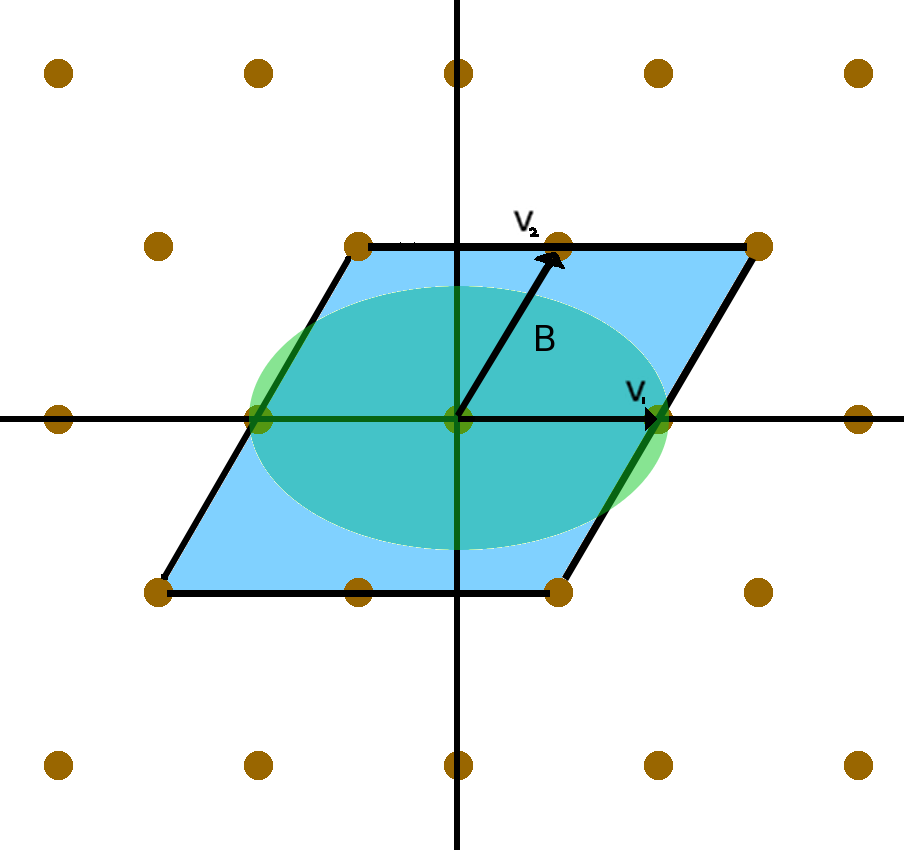
\includegraphics[width=2in]{Triangular_point_lattice}
\caption{Example \pgram{}s, $\L$, and $B$.}
\label{circlelattice}
\end{figure}

Looking at the plane (which is easier to visualize, as in Figure~\ref{circlelattice}), it is possible to make a \pgram{} that is just slightly smaller than 4 of the basic \pgram{}s tiled together and contains no nonzero lattice points. (The basic \pgram{} is just the one bounded by the basis vectors.) In $n$ dimensions, this is generalized to the \ptope{} with volume $2^n|\det(\vec v_1,\dots,\vec v_n)|$.

However, strange things can happen to the fundamental \ptope, since a lattice can have multiple $\Z$-bases. For example, $\left\{\binom{1}{0},\binom{0}{1}\right\}$ and $\left\{\binom{1}{1},\binom{1}{2}\right\}$ both represent the lattice $\Z^2$. A lattice is invariant under any change-of-basis matrix $T\in M_2(\Z)$ provided that $T^{-1}$ has integer entries. Thanks to some nice properties of $\Z$, this is equivalent to $\det T = \pm 1$, or that $T\in\GL{2}(\Z)$.
\begin{defn}
If $\{\vec v_1,\dots,\vec v_n\}$ is a $\Z$-basis of a lattice $\L\subset\R^n$, then a fundamental \ptope{} with respect to $\L$ is 
\[P = P_{\{\vec v_1,\dots,\vec v_n\}} = \left\{\sum_{i=1}^n t_i\vec v_i\mid 0\le t_i\le 1\right\}.\]
This \ptope{} and its translates cover $\R^n$.
\begin{claim}
All fundamental \ptope{}s of a given lattice have the same volume, called $\vol_{\L}$.\footnote{Notice this is not the volume \emph{of} $\!\L$, which is 0, because it is a discrete lattice.}
\end{claim}
\begin{proof}
Suppose $P$ is a fundamental \ptope{} corresponding to a basis $\{\vec v_1,\dots,\vec v_n\}$ for some lattice $\L$ and $P'$ is another fundamental \ptope{} corresponding to a basis $\{\vec v_1',\dots,\vec v_n'\}$ of $\L$. Then, there is some change-of-basis matrix $C$ such that $|\det C| = 1$. Then,
\[\vol P = |\det(\vec v_1,\dots,\vec v_n)| = |\det(C)\det(\vec v_1',\dots,\vec v_n')| = |\det C||\det(\vec v_1',\dots,\vec v_n')| = |\det C|\vol P' =\vol P'.\qedhere\]
\end{proof}
\end{defn}
\begin{thm}[Minkowski]
\label{mink}
Suppose $\L\subset\R^n$ is a lattice and $B\subset\R^n$ is convex and symmetric around the origin. Then, if $\vol(B) > 2^n\vol_{\L}$ (which is just $\vol_{2\L}$), then $B\cap(\L-\{0\}) \ne \emptyset$.
\end{thm}
Minkowski's Theorem is applicable to the four-square problem. Take $B_p = \{\|\vec v\|^2 < 2p\}\subset\R^4$ and $\L$ as given before, so that $\vol_\L = 2p^2$. In order for the theorem to be satisfied, we want $\vol(B_p) > 16p^2$. Using the four-dimensional volume of a sphere,
\[\vol B_p = \frac{\pi^2 (2p)^2}{2} = 2\pi^2 p^2 > 16p^2\]
because $\pi^2 > 8$. Step back and see how this number-theoretic property about squares of integers rests on this completly geometric property of $\pi$, which is totally unexpected.
\begin{proof}[Proof of Minkowski's Theorem]
Consider the region $2P = \left\{\sum_{i=1}^n t_i\vec v_i: 0\le t \le 2\right\}$, and for any lattice point $\vec m = \sum_{j=1}^n m_j\vec v_j$ define
\[D_{\vec m} = 2\vec m +2P = \sum_{j=1}^n 2m_j\vec v_j +2P\]
Thus, $D_{\vec m}$ is the \ptope{} translated so that one of the corners is at $\vec m$. Thus, its volume is constant, and $\vol(D_{\vec m}) = 2^n\vol_\L$. Additionally, they tesselate, since $\vec m$ is a lattice point: $\R^n = \bigcup_{\vec m\in\L} D_{\vec m}$, and they basically don't intersect (the intersections are hyperplanes with measure 0). Thus, $B\cap D_{\vec m}$ are also essentially disjoint, so since $B = \cup(B\cap D_{\vec m})$, then
\[\vol B = \sum_{\vec m}\vol(B\cap D_{\vec m}) > \vol 2P\]
by the original assumption. Now, it is possible to translate each of these pieces back to the origin, within the \ptope{} $2P$:
\[\implies \bigcup_{\vec m\in\L}(-2\vec m +(B\cap D_{\vec m})) \subseteq 2P.\]
\begin{figure}[h]
\centering
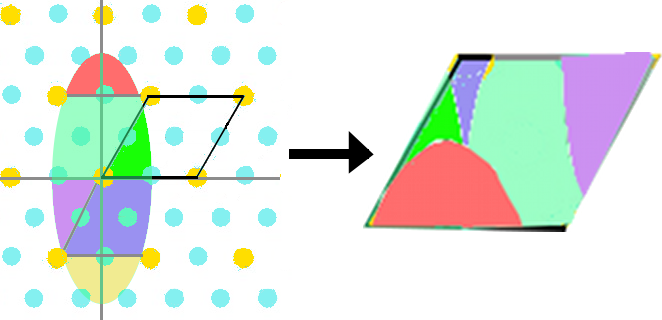
\includegraphics[height=2in]{lattice2}
\caption{Translating $B$ back to the origin to create an intersection.}
\end{figure}
But since these pieces have volume greater than $2P$, there must be distinct $\vec m$, $\vec m'$ with a nontrivial intersection: $-2\vec m + x = -2\vec m' + x'$, with $\vec m,\vec m'\in\L$ and for some $x,x'\in B$. Thus, $\frac{x'-x}{2} = \vec m'-\vec m$, which is also a nonzero lattice point (since $\vec m'$ and $\vec m$ are distinct) that is in $B$ (by symmetry, since $x$ is, then so is $-x$, and by convexity, their midpoint is as well).
\end{proof}
The four-squares theorem follows as above.
\end{proof}
A lot of problems in number theory, such as those relating to the theory of quadratic forms, can be solved in similar ways.
%a\end{document}
